\subsection{Κατανόηση Αλγορίθμου}
Η μέθοδος του χρυσού τομέα διαμορφώνει διαστήματα αναζήτησης τα οποία είναι αναλογικά μεταξύ τους.
Συγκεκριμένα ο λόγος μεταξύ δύο διαδοχικών χωρίων είναι ίσος με την σταθερά γ. Ένα κομμάτι στο 
οποίο η μέθοδος αυτή βελτιώνει την μέθοδο της διχοτόμησης είναι ότι μετά την πρώτη φορά που
υπολογίζει τις τιμές της συνάρτησης τις επόμενες επαναλήψεις χρειάζεται να υπολογίσει μόνο
μία τιμή της συνάρτησης. 

\subsection{Υπολογισμοί αντικειμενικής συνάρτησης συναρτήσει του $l$}

\begin{figure}[H] % h for 'here', you can also use t (top), b (bottom), or p (page)
    \centering
    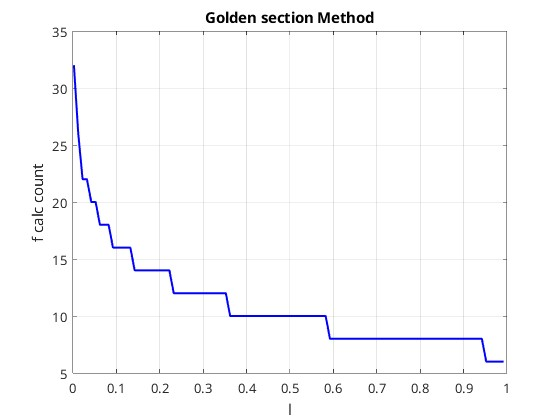
\includegraphics[width=0.5\textwidth]{media/goldenf1} % Image file without extension
    \caption{Συνάρτηση $f_1$}
\end{figure}

\begin{figure}[H] % h for 'here', you can also use t (top), b (bottom), or p (page)
    \centering
    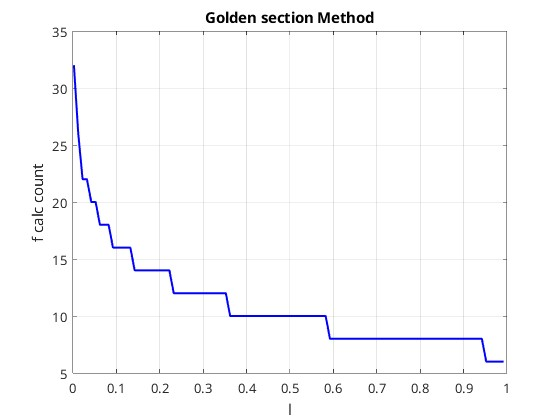
\includegraphics[width=0.5\textwidth]{media/goldenf2} % Image file without extension
    \caption{Συνάρτηση $f_2$}
\end{figure}

\begin{figure}[H] % h for 'here', you can also use t (top), b (bottom), or p (page)
    \centering
    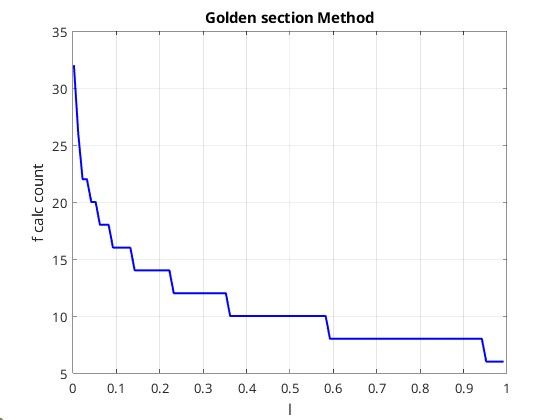
\includegraphics[width=0.5\textwidth]{media/goldenf3} % Image file without extension
    \caption{Συνάρτηση $f_3$}
\end{figure}

\subsection{Άκρα του διαστήματος αναζήτησης συναρτήσει του δείκτη επαναλήψεων}
Συνάρτηση $f_1$:
\begin{figure}[H] % h for 'here', you can also use t (top), b (bottom), or p (page)
    \centering
    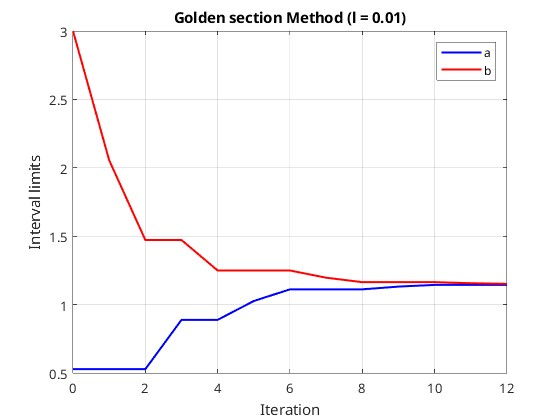
\includegraphics[width=0.5\textwidth]{media/goldenf1_001} % Image file without extension
    \caption{Συνάρτηση $f_1$}
\end{figure}
\begin{figure}[H] % h for 'here', you can also use t (top), b (bottom), or p (page)
    \centering
    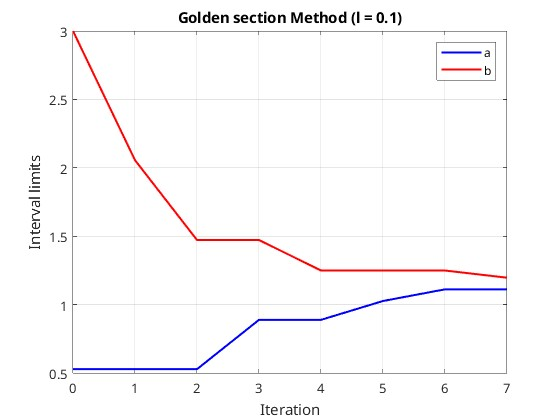
\includegraphics[width=0.5\textwidth]{media/goldenf1_01} % Image file without extension
    \caption{Συνάρτηση $f_1$}
\end{figure}
\begin{figure}[H] % h for 'here', you can also use t (top), b (bottom), or p (page)
    \centering
    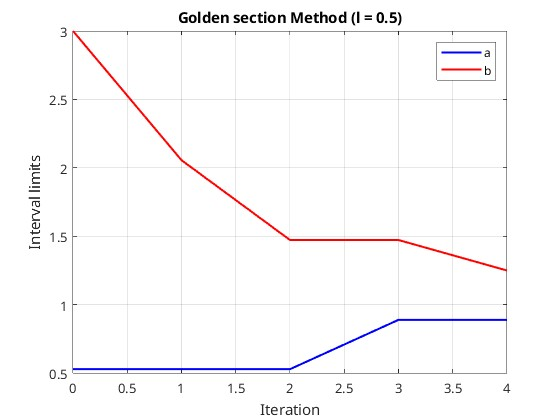
\includegraphics[width=0.5\textwidth]{media/goldenf1_05} % Image file without extension
    \caption{Συνάρτηση $f_1$}
\end{figure}

Συνάρτηση $f_2$:
\begin{figure}[H] % h for 'here', you can also use t (top), b (bottom), or p (page)
    \centering
    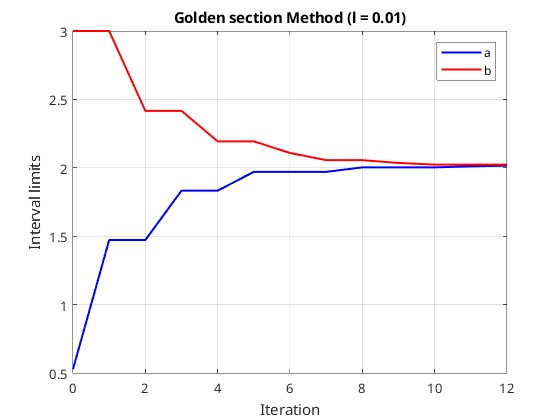
\includegraphics[width=0.5\textwidth]{media/goldenf2_001} % Image file without extension
    \caption{Συνάρτηση $f_2$}
\end{figure}
\begin{figure}[H] % h for 'here', you can also use t (top), b (bottom), or p (page)
    \centering
    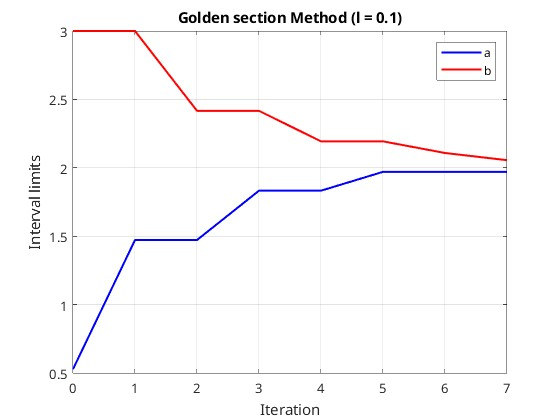
\includegraphics[width=0.5\textwidth]{media/goldenf2_01} % Image file without extension
    \caption{Συνάρτηση $f_2$}
\end{figure}
\begin{figure}[H] % h for 'here', you can also use t (top), b (bottom), or p (page)
    \centering
    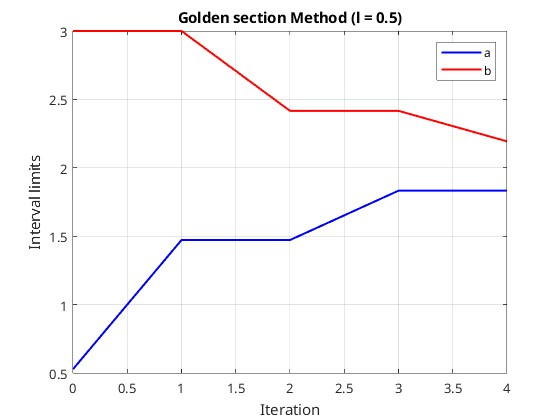
\includegraphics[width=0.5\textwidth]{media/goldenf2_05} % Image file without extension
    \caption{Συνάρτηση $f_2$}
\end{figure}

Συνάρτηση $f_3$:
\begin{figure}[H] % h for 'here', you can also use t (top), b (bottom), or p (page)
    \centering
    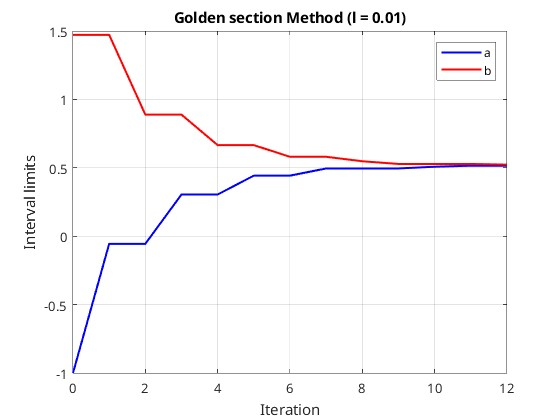
\includegraphics[width=0.5\textwidth]{media/goldenf3_001} % Image file without extension
    \caption{Συνάρτηση $f_3$}
\end{figure}
\begin{figure}[H] % h for 'here', you can also use t (top), b (bottom), or p (page)
    \centering
    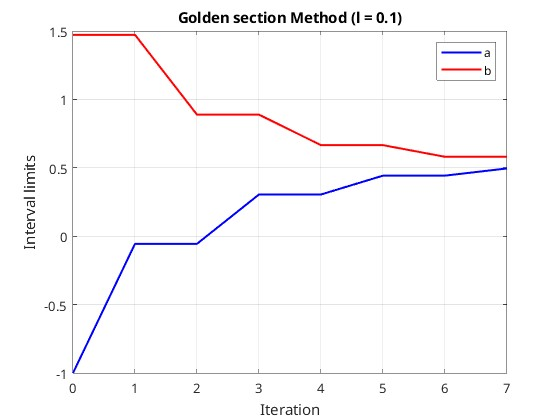
\includegraphics[width=0.5\textwidth]{media/goldenf3_01} % Image file without extension
    \caption{Συνάρτηση $f_3$}
\end{figure}
\begin{figure}[H] % h for 'here', you can also use t (top), b (bottom), or p (page)
    \centering
    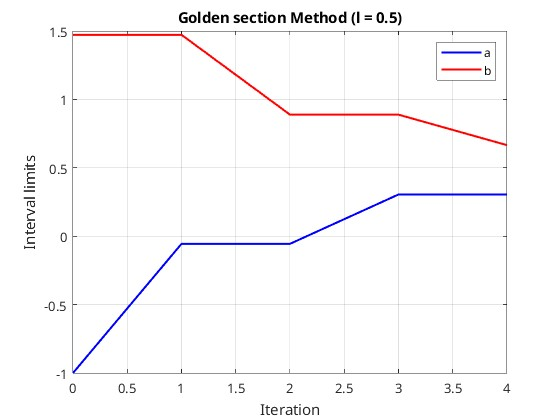
\includegraphics[width=0.5\textwidth]{media/goldenf3_05} % Image file without extension
    \caption{Συνάρτηση $f_3$}
\end{figure}